% - Vous en avez déjà parlé avec les autres profs?
% - Qui a peur ? [exprimez-vous!]
%   je reformule:
%   - peur d'attraper?
%   - peur de transmettre à un proche fragile
% - Qui pense que gnognotte/complot?
%   => si conflit => "je vois avis divergents => discuter (aux pauses, n'hésitez pas à me contacter même si je suis pas médecin)"
%   => si pas conflit => c'est pas un cours sur le COVID => [cf. au-dessus]...

\documentclass[french,c,xcolor={pdftex,svgnames}, % dvipsnames, dvipsnames*, svgnames, svgnames*, x11names,
]{beamer}  %
\usetheme{Copenhagen}

% Remove navigation bar
\setbeamertemplate{navigation symbols}{}
% Remove outline at top
\setbeamertemplate{headline}{}

% For links
\usepackage{hyperref}
% PDF settings
\hypersetup{%
  pdftitle={Rappels COVID-19},%
  pdfauthor={Guillaume MULLER},%
  pdfsubject={COVID-19},%
  pdfkeywords={COVID-19},%
  colorlinks=true,%
  urlcolor=blue,%
  linkcolor=%
}

% Correct French/English indentation and splitting of words
\usepackage{babel}

% Correct management of accentuated chars in input file
\usepackage[utf8]{inputenc}
%\usepackage[utf8]{inputenc}

% Correct font for the generation of docs with accentuated chars
\usepackage[T1]{fontenc}      % Can handle hyphenation of words with accented characters

% Multi-row in tabulars
\usepackage{multirow}

% Insertion of images generated by external tools
\usepackage{graphicx}

% For graphics
\usepackage{tikz}
\usetikzlibrary{calc}


\def\slider#1#2#3#4{% 1: length / 2: position of the mark (0 to 1) / 3: start color / 4: end color
  \shorthandoff{:!} % protection in french babel mode
  \tikz[baseline=0cm]{
    \coordinate (start) at (0,0);
    \coordinate (end) at (#1,0);
    \coordinate (mark) at ($(start)!#2!(end)$);
    \fill[left color=#3, right color=#4, fill, shading angle=95, rounded corners] (start)[above=.7em] rectangle (end)[below=.7em] ;
    \path[
        fill=blue!30!cyan,
    ] (mark) + (-.3em, -.2em) -- +(0em, -.4em) -- +(.3em, -.2em) -- +(.3em, .9em) -- +(-.3em, .9em) -- cycle;
  }
  \shorthandon{:!}
}

\def\redcross#1#2{
  \begin{tikzpicture}
    \node (img) {\includegraphics[height=#1]{#2}};
    \draw[red, line width=.5ex]
    (img.south west) -- (img.north east)
    (img.south east) -- (img.north west);
  \end{tikzpicture}
}

%%%%%%%%%%%%%%%%%%%%%%%%%%%%%%%%%%%%%%%%%%%%%%%%%%%%%%%%%%%%%%%%%%%%%%
\begin{document}

\title{COVID Rules}
\author{Guillaume \textsc{Muller}}
%\date

\begin{frame}
  \maketitle
\end{frame}


%%%%%%%%%%%%%%%%%%%%%%%%%%%%%%%%%%%%%%%%
\def\imagetop#1{\vtop{\null\hbox{#1}}}
\begin{frame}{Rappels COVID-19 - Current Knowledge}

    \begin{itemize}
      \item<1-4>[] \hspace{3cm} \raisebox{-.45\height}{
\includegraphics[width=5em]{images00/dont-panic.png}} % Generally showning don't panic sign => people panics
      \vspace*{.5cm}
%
      \item<2-4>[] \raisebox{-.45\height}{
\includegraphics[width=3em]{images00/thumb_up.png}}
        $\Rightarrow$ \raisebox{-.45\height}{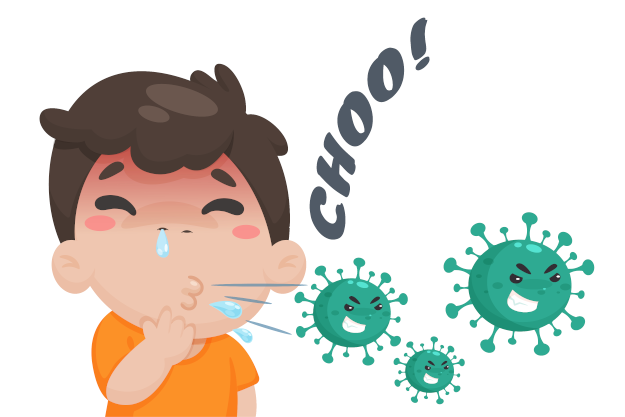
\includegraphics[width=5em]{images00/sneeze.png}}
      \vspace*{.2cm}
      \item<3-4>[] \raisebox{-.45\height}{
\includegraphics[width=3em]{images00/thumb_down.png}}
        $\Rightarrow$
        \raisebox{-.45\height}{
\includegraphics[width=3em]{images00/seringe1.png}}
        \raisebox{-.45\height}{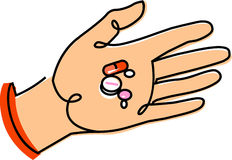
\includegraphics[width=3em]{images00/pills.jpg}}
        $\Rightarrow$
        \raisebox{-.45\height}{\rotatebox{90}{\resizebox{2em}{!}{\slider{5em}{0.7}{black}{black}}}}
        \raisebox{-.45\height}{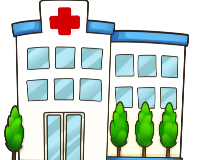
\includegraphics[width=3em]{images00/clinic.png}}
        \vspace*{.5cm}
%
        \item<4>[] { \tiny \hspace*{-2.4em}\begin{tabular}{cl}
          \multirow{2}{*}{
            \imagetop{
\includegraphics[width=4.5em]{images00/news.png}}
          }
          & \\
          & \url{https://www.univ-st-etienne.fr/fr/faq-rentree-2020-2021/informations-generales.html} \\
          & \url{https://www.univ-st-etienne.fr/fr/info-coronavirus/videos-sur-ce-sujet.html} \\
          & \url{brigitte.poizat@univ-st-etienne.fr} \\
        \end{tabular}
      }
        \item<4>[] ~\\[.3em]
        \begin{center}
          \raisebox{-.45\height}{\redcross{1em}{images00/Facebook.png}}
          \raisebox{-.45\height}{\redcross{1em}{images00/Twitter.png}}
          \raisebox{-.45\height}{\redcross{1em}{images00/Instagram.png}}
        \end{center}
      \end{itemize}
% Le service hygiène et sécurité : sandrine.cazaubon@univ-st-etienne.fr
% La médecine préventive : brigitte.poizat@univ-st-etienne.fr

\end{frame}


%%%%%%%%%%%%%%%%%%%%%%%%%%%%%%%%%%%%%%%%
\begin{frame}{Rappels COVID-19 - National/TSÉ rules}

  \begin{itemize}
    \item[] \raisebox{-.45\height}{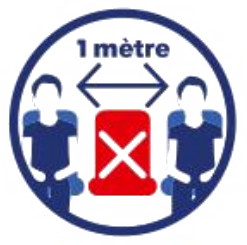
\includegraphics[width=2.5em]{images00/distance.png}} \hspace{.3cm}
      Garder les \textbf{distances} { \scriptsize ($>$1~m) }
    \item[] \raisebox{-.45\height}{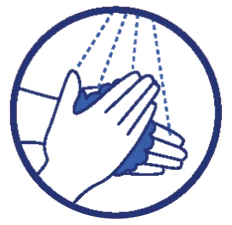
\includegraphics[width=2.5em]{images00/lavage_mains.png}} \hspace{.3cm}
      Se laver régulièrement les \textbf{mains} { \scriptsize ($\approx$30 min.) }
    \item[] \raisebox{-.45\height}{
\includegraphics[width=2.5em]{images00/masque.png}} \hspace{.3cm}
      Mettre un \textbf{masque} { \scriptsize (intérieur+dense, \textbf{nez}+bouche) }
    \item[] \raisebox{-.45\height}{
\includegraphics[width=2.5em]{images00/windows10.png}} \hspace{.3cm}
      Ouvrir les \textbf{fenêtres} régulièrement { \scriptsize ($\approx$3 hr.)}
  \end{itemize}

\end{frame}

%%%%%%%%%%%%%%%%%%%%%%%%%%%%%%%%%%%%%%%%
\begin{frame}{Rappels COVID-19 - Help me!}

  \begin{center}
    \onslide<1->{ \bigskip COOL \slider{10em}{0.7}{blue}{red} PARANO }
    \bigskip
    \onslide<2>{ 
\includegraphics[width=10em]{images00/raising-hands.png} }
  \end{center}

\end{frame}

\end{document}


%%% Local Variables:
%%% mode: latex
%%% TeX-master: t
%%% End:
